\documentclass{article}

\usepackage{graphicx}
\usepackage{tikz}
\usepackage{tikzsymbols}
\usetikzlibrary{calc,patterns,shapes.geometric}
\pagestyle{empty}
\usepackage[margin=0pt]{geometry}
\geometry{papersize={14in,12in}}

\def\centerarc[#1](#2)(#3:#4:#5){\draw[#1] ($(#2)+({#5*cos(#3)},{#5*sin(#3)})$) arc (#3:#4:#5);}

\begin{document}
	\begin{figure}
		\centering
		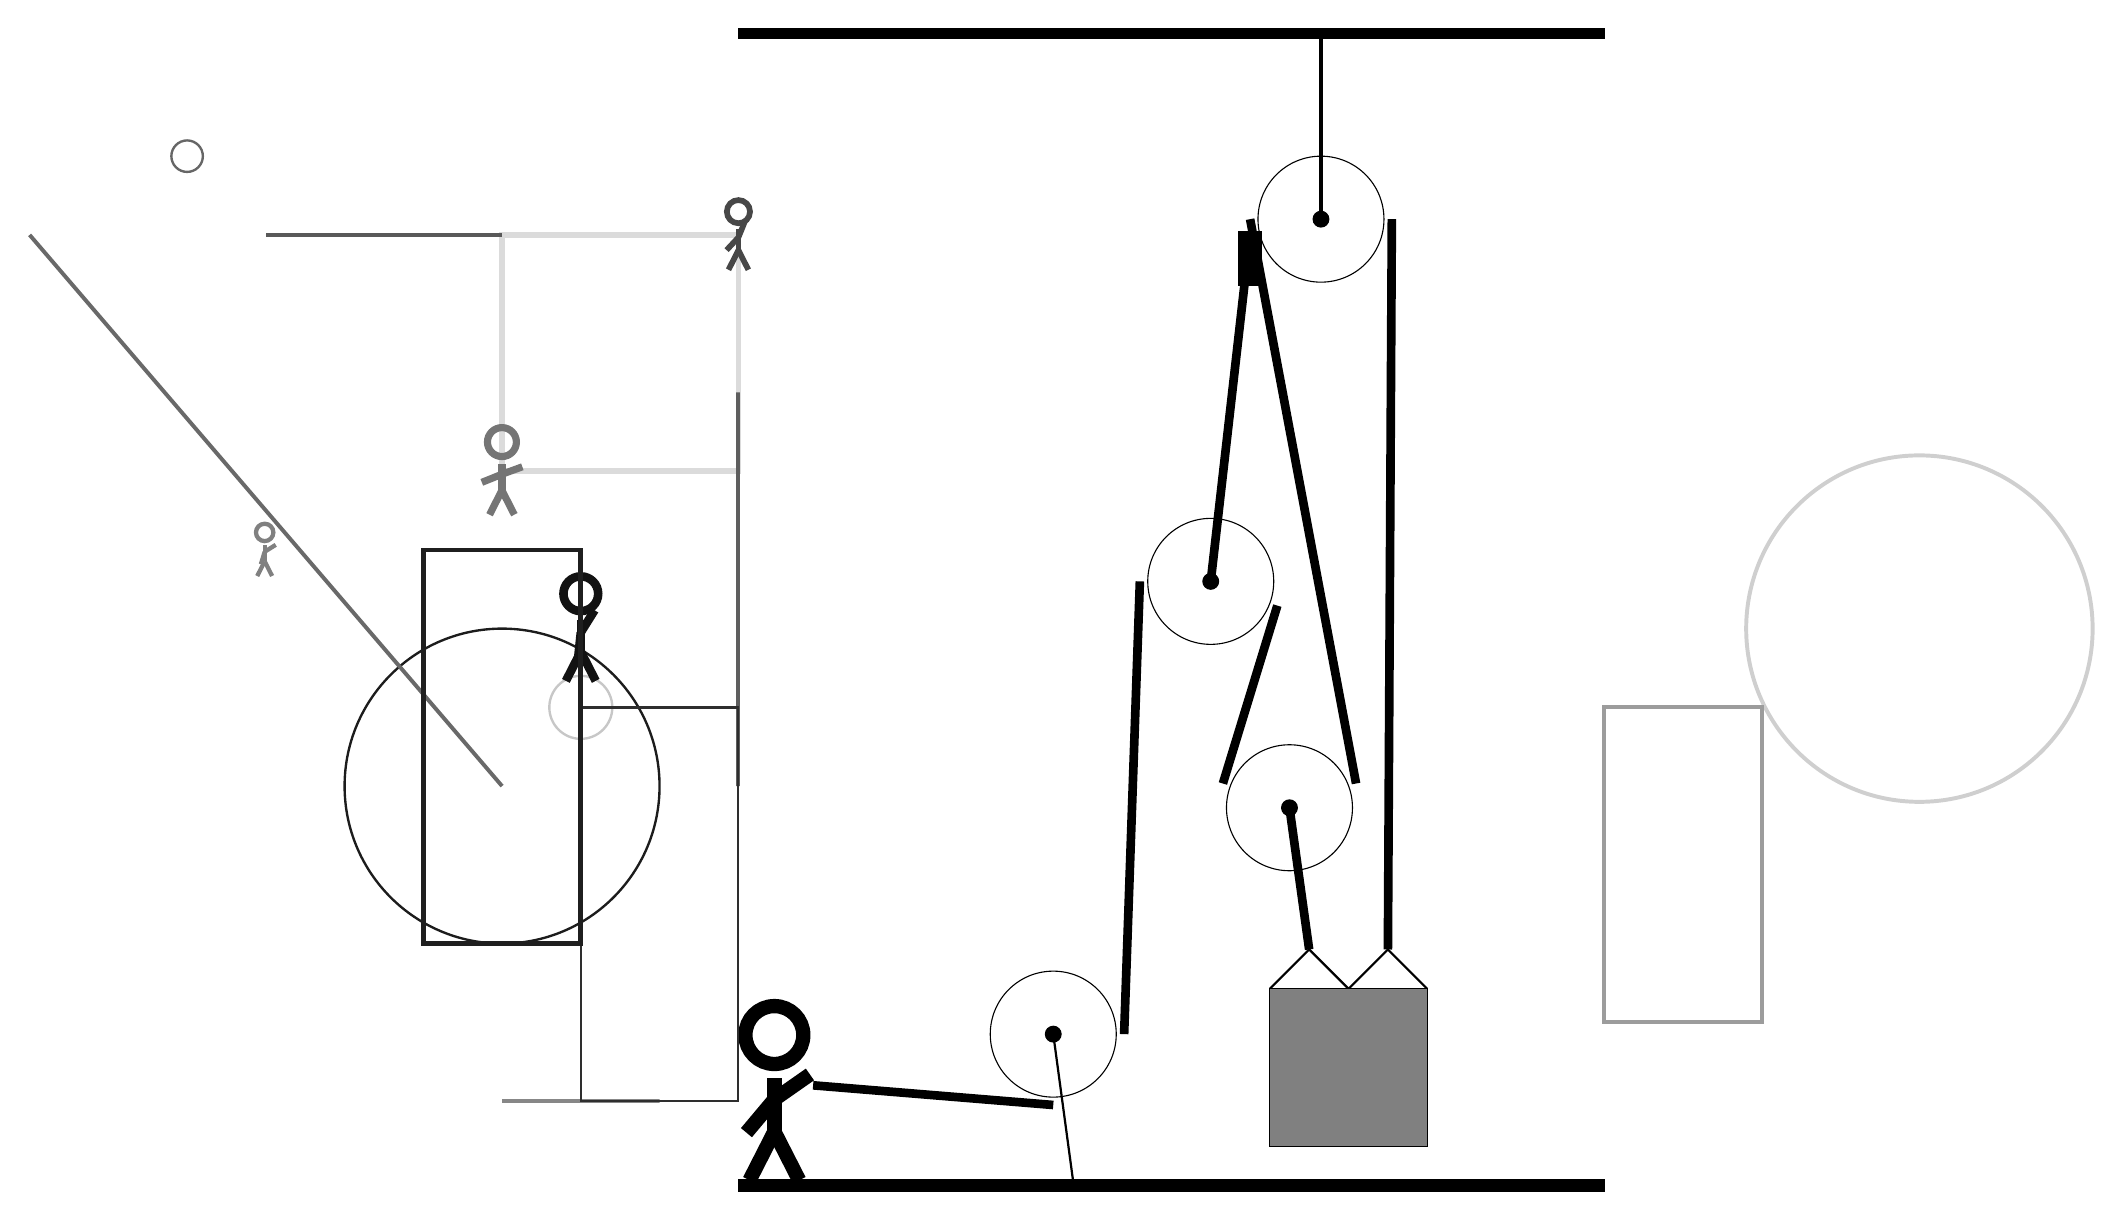
\begin{tikzpicture}
			%%%%% START %%%%%
			
			\draw[fill=black] (-6, 11.5) rectangle (5, 11.625);
			
			\draw (0, 4.6) circle (0.8);
			\draw[fill=black] (0, 4.6) circle (0.1);
			
			\draw (1, 1.725) circle (0.8);
			\draw[fill=black] (1, 1.725) circle (0.1);
			
			\draw (1.4, 9.2) circle (0.8);
			\draw[fill=black] (1.4, 9.2) circle (0.1);
			\draw[very thick] (1.4, 9.2) -- (1.4, 11.5);
			
			\draw (-2, -1.15) circle (0.8);
			\draw[fill=black] (-2, -1.15) circle (0.1);
			\draw[thick] (-2, -1.15) -- (-1.75, -3);
			
			
			\draw[thick]  (0.75, -0.575) -- (1.25, -0.075) -- (1.75, -0.575) -- (2.25, -0.075) -- (2.75, -0.575);
			\draw[fill=black!50] (0.75, -0.575) rectangle (2.75, -2.575);
			\draw[line width=1.1mm] (-5.05, -1.8) -- (-2, -2.05);
			\centerarc[line width=1.1mm](-2, -1.15)(270:360:0.9);
			\draw[line width=1.1mm] (-1.1, -1.15) -- (-0.9, 4.6);
			\draw[line width=1.1mm] (0, 4.6) -- (0.5, 9.0);
			\draw[line width=1.1mm, fill=black](0.4, 8.4) rectangle (0.6, 9.0);
			\centerarc[line width=1.1mm](0, 4.6)(-20:180:0.9);
			\draw[line width=1.1mm] (0.8457, 4.2922) -- (0.1543, 2.0328);
			\centerarc[line width=1.1mm](1, 1.725)(160:380:0.9);
			\draw[line width=1.1mm] (1.8457, 2.0328) -- (0.5, 9.2);
			\draw[line width=1.1mm](1, 1.725) -- (1.25, -0.075);
			\centerarc[line width=1.1mm](1.4, 9.2)(0:180:0.9);
			\draw[line width=1.1mm] (2.3, 9.2) -- (2.25, -0.075);
			
			\node at (-5.5, -1.9) {\Strichmaxerl[10][50][35]};
			
			\draw [line width=0.3mm, color=black!60](-13, 10) circle (0.2);
			
			\draw [line width=0.3mm, color=black!22](-8, 3) circle (0.4);
			\draw[line width=0.7mm, color=black!14] (-6, 6) rectangle (-9, 9);
			\node[line width=0.2mm, color=black!54] at (-9, 6) {\Strichmaxerl[5][22][20]};
			
			\draw [line width=0.3mm, color=black!89](-9, 2) circle (2.0);
			\node[line width=0.3mm, color=black!50] at (-12, 5) {\Strichmaxerl[3][73][32]};
			
			\draw[line width=0.5mm, color=black!65](-9, 9) -- (-12, 9);
			\draw[line width=0.5mm, color=black!59](-9, 2) -- (-15, 9);
			\draw [line width=0.5mm, color=black!19](9, 4) circle (2.2);
			
			\draw[line width=0.5mm, color=black!39] (5, -1) rectangle (7, 3);
			\node[line width=0.6mm, color=black!93] at (-8, 4) {\Strichmaxerl[6][84][58]};
			
			\draw[line width=0.6mm, color=black!47] (-7, -2) rectangle (-9, -2);
			\node[line width=0.5mm, color=black!72] at (-6, 9) {\Strichmaxerl[4][47][68]};
			
			\draw[line width=0.5mm, color=black!63] (-6, 7) rectangle (-6, 2);
			\draw[line width=0.3mm, color=black!82] (-6, 3) rectangle (-8, -2);
			\draw[line width=0.6mm, color=black!88] (-8, 5) rectangle (-10, 0);
			
			
			\draw[fill=black] (-6, -3) rectangle (5, -3.15);
			
			%%%%% END %%%%%
		\end{tikzpicture}
	\end{figure}	
\end{document}